\chapter{Design}
\subsection{<for mobiles>}
when designing a mobile app with UX focus, the unique challenges of the mobile platform has to be considered. A brief look at three of the most outstanding challenges:
\begin{itemize}
\item Screen size\\
as opposed to a traditional computer screen the general mobile platform has a much more limited amount of screen space. This restriction will force the designers to eliminate as many redundancies as possible so as to not clutter the screen with unnecessary information. \cite{Sardo}
\item User input\\
user input is according to Giorgio Sardo one of  the smartphones weakness. it is mentioned that “Entering text on a mobile phone is hard, and people tend to avoid it if they can”\cite{Sardo}
\item Loading times\\
Mobile devices are generally slower than a PC or Mac, both when it comes to processing power and internet speed, assuming they’re using a mobile network \cite{MobileUsability}
\end{itemize}

Some of the guidelines for optimizing for mobile devices are cutting features, reduce word count and enlarge interface elements to accommodate the “fat finger problem”.\cite{MobileUsability} an example of poor simplification used in the book is IKEA where they simplify the mobile site by only showing a single item when browsing for bedframes.

\begin{figure}[H]
\centering
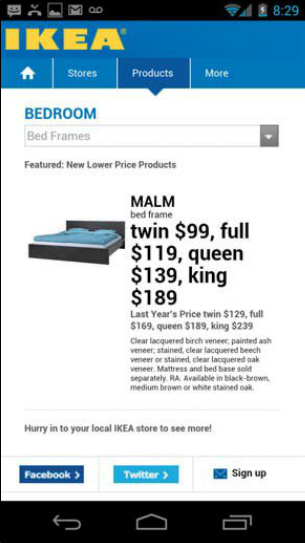
\includegraphics[scale=0.5]{IkeaBadMobile.png}
\caption{the mobile website from IKEA, anno 2013}
\end{figure}